%%
%% LaTeX Document Template
%%
\documentclass[sigplan,screen]{acmart}
%%
%% \BibTeX command to typeset BibTeX logo in the docs
\AtBeginDocument{%
  \providecommand\BibTeX{{%
    Bib\TeX}}}

%% Publication information - modify as needed
\setcopyright{none}
\acmConference[]{University of Auckland}{University of Auckland}{2025}

%% Citation style configuration
\citestyle{acmauthoryear}


%%
%% Additional packages for figures and subfigures
\usepackage{graphicx}
\usepackage{subcaption}
\usepackage{pifont}

%%
%% Hyperref is automatically loaded by acmart class
%% Configure colors for links
\hypersetup{
    colorlinks=true,
    linkcolor=blue,
    citecolor=red,
    urlcolor=cyan
}

%%
%% end of the preamble, start of the body of the document source.
% Improve line breaking to avoid overfull boxes for long words
\emergencystretch=3em
\begin{document}

%%
%% The "title" command has an optional parameter,
%% allowing the author to define a "short title" to be used in page headers.
\title[LumineticsCore Report]{Lifecycle Governance and Value Assessment of an FDA De Novo--Authorized Autonomous Diagnostic System: The LumineticsCore Report}

%% Author information
\author{Xiaoqing Miao}
\email{xmia665@aucklanduni.ac.nz}
\affiliation{%
  \institution{University of Auckland }
  \city{Auckland}
  \country{New Zealand}
}


%% Short author list for page headers
\renewcommand{\shortauthors}{Xiaoqing Miao}

%%
%% This command processes the author and affiliation and title
%% information and builds the first part of the formatted document.
\maketitle

\section{Introduction and Scope}

\subsection{System Definition}

LumineticsCore is the first autonomous Artificial Intelligence (AI) medical device granted De Novo authorization (2018, DEN180001) by the U.S. Food and Drug Administration (FDA) that can provide a diagnostic and management recommendation at the point of care without interpretation by a human expert, designed to address the bottlenecks of coverage and timeliness in diabetic retinopathy (DR) screening within primary care settings.

Diabetic retinopathy (DR) is a major cause of preventable blindness, but in the traditional referral-based workflow of primary care or community clinics, examinations are difficult to complete in a timely manner and patient adherence is low, leading to delays in treating manageable conditions \cite{wolf2024autonomous}. LumineticsCore (formerly IDx-DR) is an autonomous AI diagnostic system authorized via FDA De Novo \cite{fda2018denovo} that analyzes color fundus photographs of patients with diabetes at the point of care to automatically determine if the condition has reached ``more-than-mild diabetic retinopathy (mtmDR),'' which is defined as a level $\geq$35 on the Early Treatment Diabetic Retinopathy Study (ETDRS) scale and/or the presence of diabetic macular edema (DME), and based on this, outputs an actionable management recommendation (refer/rescreen/retake) to enhance the accessibility and timeliness of screening \cite{digitaldiagnostics2024indications}.

\subsection{Target Users and Expected Clinical Outcomes}

The target users for LumineticsCore are non-ophthalmic healthcare professionals (such as nurses or technicians) in primary care settings \cite{digitaldiagnostics2024indications}, and its intended patient population is diabetic adults aged 22 and older who have been diagnosed with diabetes but have no prior history of DR \cite{fda2018denovo_summary}.

The system's core clinical workflow is designed to be exceptionally simple. After the operator uses the accompanying Topcon TRC-NW400 camera to capture images according to the specified protocol (one 45° color photograph centered on the macula and one on the optic disc for each eye), the system immediately returns one of three clear, actionable management recommendations:

\textbf{Positive Finding}: If the result is determined to be ``more-than-mild diabetic retinopathy (mtmDR),'' an immediate referral to an eye care specialist is recommended.

\textbf{Negative Finding}: If the result is negative, the recommendation is to rescreen in 12 months.

\textbf{Insufficient Quality}: If the images cannot be analyzed, the operator is prompted to retake them. If the images are still of insufficient quality after retakes, the patient is likewise referred according to the protocol \cite{fda2018denovo_summary}.

The system's expected clinical value lies in breaking down the barriers of delay and loss to follow-up inherent in traditional screening models, which are caused by waiting and appointment scheduling, thereby significantly increasing the completion rate of eye exams and accelerating necessary referrals. The effectiveness of this mechanism has been powerfully demonstrated in a randomized controlled trial involving a multi-ethnic adolescent population: with AI assistance, the completion rate of eye exams within 6 months was 100\%, far exceeding the 22\% rate of the conventional referral group \cite{wolf2024autonomous}. Although this study population differs from the system's labeled adult users, it provides strong supporting evidence for the core hypothesis that point-of-care diagnostics improve treatment adherence.

\subsection{Evaluation Scope and Boundaries}

To ensure the precision and depth of the analysis, the scope of this report will strictly focus on the core autonomous diagnostic function of LumineticsCore. Its specific boundaries adhere to the system's regulatory-approved labeling and the evaluation requirements of this course. The scope is defined in detail as follows:

\textbf{Functional Scope}: The evaluation is limited to the system's core capability of autonomously determining whether the threshold for ``more-than-mild diabetic retinopathy (mtmDR)'' has been met based on standard fundus photographs and outputting a corresponding management recommendation. Any functions aiding therapeutic decisions are excluded from this discussion \cite{fda2018denovo_summary}.

\textbf{Contextual Scope}: The evaluation is set within the workflow of a single visit at a primary care institution (check-in $\rightarrow$ imaging $\rightarrow$ analysis $\rightarrow$ communication $\rightarrow$ disposition). The user is assumed to be a non-ophthalmic healthcare professional who has undergone the minimum necessary training \cite{digitaldiagnostics2024indications}.

\textbf{Technical Scope}: The input data is limited to one 45° color photograph centered on the macula and one on the optic disc for each eye, acquired by a Topcon TRC-NW400 camera. The system utilizes a client-server architecture, requiring an internet connection to send images to a controlled data center (including a web front-end, database, logs, and network security) for analysis. Imaging is typically performed without mydriasis (pupil dilation), although dilation may be used when necessary to improve the image acquisition rate \cite{fda2018denovo_summary}.

\textbf{Population Scope}: The applicable population is strictly limited to diabetic adult patients aged 22 and older with a confirmed diagnosis of diabetes and no prior history of DR. Potential applications for children/adolescents, other imaging devices/protocols, or non-DR eye diseases (such as glaucoma or Age-related Macular Degeneration, AMD) are not within the scope of this evaluation \cite{fda2018denovo_summary}.

\subsection{Methodology}

This report employs a single-case evidence summary and standardized evaluation method to systematically analyze the autonomous diagnostic system LumineticsCore (formerly IDx-DR). The research adheres to the principle of reproducibility, with the methodology as follows:

\textbf{(1) Research Question and Scope}

The focus is on the efficacy, safety, usability, and explainability of the system for screening ``more-than-mild diabetic retinopathy (mtmDR)'' in a primary care setting. Only the core autonomous diagnostic function is evaluated; therapeutic decision-making and non-DR diseases are not addressed.

\textbf{(2) Evidence Sources and Search Strategy}

A comprehensive review of regulatory documents (FDA De Novo decision letters and subsequent 510(k) summaries/database entries), peer-reviewed literature (pivotal trials, randomized/quasi-randomized and real-world studies), official instructions for use/indication pages, and course reading lists was conducted. Keywords were searched in PubMed, Scopus, and Web of Science: ``IDx-DR OR LumineticsCore AND (diabetic retinopathy OR mtmDR) AND (trial OR randomized OR real-world OR De Novo OR 510(k))''. The search was limited to the English language (supplemented with manufacturer documentation where necessary), with a search cut-off date of October 5, 2025 (NZT).

\textbf{(3) Inclusion and Exclusion Criteria}

Inclusion criteria were: \ding{172} Regulatory documents directly related to LumineticsCore; \ding{173} Peer-reviewed studies reporting original data or pre-specified outcomes (pivotal trials, RCTs, cluster-randomized/real-world studies); \ding{174} Official indications/instructions for use. Exclusion criteria were: press releases, opinion-based editorials, and secondary reviews without a direct evidence link to the system (except for background information).

\textbf{(4) Evidence Quality and Reporting Adequacy Assessment}

The reporting transparency and protocol adequacy of clinical studies were checked against the CONSORT-AI and SPIRIT-AI guidelines. The QUADAS-2 tool was used to assess the risk of bias and applicability of diagnostic accuracy studies. The RoB 2 tool was referenced for randomized studies. Where necessary, the GRADE approach was used to roughly classify the strength of evidence for key outcomes.

\textbf{(5) Data Extraction and Synthesis}

Key data extracted included: primary performance metrics (sensitivity, specificity, imageability rate, predictive values; F1/ROC if available), use case context and population, input and device specifications, output and management recommendations, and human factors/training and cybersecurity requirements. Data were synthesized descriptively, primarily through comparison with clinical guidelines and regulatory limitations, maintaining an interpretive boundary ``consistent with the indication for use.''

\textbf{(6) Usability and Interaction Assessment Method}

Nielsen's ten usability heuristics (e.g., visibility of system status, consistency, error prevention, recognition rather than recall) served as the primary framework \cite{nielsen2020usability}. A heuristic walkthrough was conducted based on publicly available interface/workflow descriptions and regulatory ``human factors validation'' entries. Where feasible, this was supplemented by a small-sample System Usability Scale (SUS) score (as qualitative support, not for inferential statistics).

\textbf{(7) Explainability/Reverse-Engineering Method}

Based on the public labeling and workflow, a simplified decision tree was constructed as an action-level proxy model (``Quality Gate $\rightarrow$ Lesion Detection $\rightarrow$ Comparison with mtmDR Threshold $\rightarrow$ Three Output/Action Categories''). This was used to illustrate how system outputs map to executable clinical dispositions, explicitly clarifying it as a proxy for explanatory purposes and not the manufacturer's internal algorithm.

\textbf{(8) Ethics and Compliance Statement}

This report is a secondary analysis based solely on publicly available information and does not involve new human subject research. All cited clinical studies have reported IRB approval, informed consent, and arrangements such as model locking/third-party escrow in their original publications (which was verified during the evidence quality assessment).

\textbf{(9) Limitations}

Potential risks include publication bias and selective reporting due to manufacturer-affiliated authors. The heterogeneity of real-world device versions and workflows limits generalizability. There is limited evidence for the re-validation of the model's performance after updates. These uncertainties will be discussed in the reflection in Section 6.

\section{Source and Knowledge Base}

\subsection{Knowledge Source and Task Boundaries}

The knowledge base of LumineticsCore (formerly IDx-DR) originates from a large dataset of fundus images (exact scale undisclosed) labeled by ophthalmology experts according to the ETDRS grading scale. The model uses deep learning (such as a Convolutional Neural Network, CNN) to learn the lesion patterns associated with mtmDR from this data, including microaneurysms, hemorrhages, hard exudates, and signs related to DME \cite{abramoff2018pivotal}. The ETDRS scale is the gold standard in clinical trials and practice for quantifying the severity of DR; therefore, the AI's ``knowledge'' is essentially the digitalized and modeled diagnostic consensus of top experts. Through deep learning algorithms (specifically CNNs), the AI learns from this labeled data to identify the complex lesion patterns associated with ``more-than-mild diabetic retinopathy (mtmDR),'' such as microaneurysms, hemorrhages, hard exudates, and diabetic macular edema.

The task boundary for this system is strictly limited to an autonomous, patient-level binary classification task. The specific workflow is as follows: the system receives images captured by a Topcon TRC-NW400 camera according to a standard protocol (one 45° color photograph centered on the macula and one on the optic disc for each eye) as its sole input. Subsequently, the AI algorithm performs an autonomous analysis. Its final output is not a detailed description of lesions or a probability score, but rather a clear, directly actionable clinical management recommendation that places the patient into one of three preset categories: refer to an eye care specialist (mtmDR positive), rescreen in 12 months (mtmDR negative), or retake images (insufficient image quality) \cite{fda2018denovo_summary}. This design clearly defines its role as a frontline screening tool, with task boundaries that do not involve disease grading, treatment recommendations, or the diagnosis of other eye diseases, thereby ensuring its safety and ease of use in the primary care setting.

\subsection{Data and Ethics: Adaptability and Clinical Validation}

The clinical adaptability and ethical compliance of LumineticsCore are not based solely on its algorithmic accuracy but are established upon a meticulously designed, prospective clinical validation process conducted in a real-world setting. This process proactively addresses the core ethical concerns of medical AI, such as Fairness, Accountability, and Transparency.

The system's pivotal trial \cite{abramoff2018pivotal} was conducted in 10 primary care (non-ophthalmology) clinics, enrolling a total of 900 patients with diabetes. The trial's design reflects the following key principles of ethics and data governance:

\begin{itemize}
\item \textbf{Addressing Bias and Ensuring Fairness:} To prevent algorithmic bias and ensure the generalizability of the results, the trial intentionally enrolled a diverse population. Data show that participants included groups of different genders, ages, and races (for example, approximately 21\% of participants were African American) \cite{abramoff2018pivotal}. This measure directly addresses a primary step in resolving AI bias---``re-examining data to ensure it represents the diverse populations served''---and aims to validate the model's robustness across different subgroups, thereby promoting health equity.

\item \textbf{Informed Consent and Accountability:} Strict ethical oversight was a cornerstone of the trial. All studies were approved by an Institutional Review Board (IRB), and every participant provided written informed consent, which protects patients' data privacy and autonomy. More critically, to ensure accountability and the integrity of the study, the trial employed an ``algorithm lock'' mechanism: before the trial began, the AI model was finalized and placed in the custody of a third-party algorithm integrity organization, and no modifications were permitted during the study \cite{fda2018denovo_summary}. This prevents potential conflicts of interest where developers might intervene mid-trial to achieve better results and establishes clear boundaries of accountability.

\item \textbf{Independent Clinical Validation and Human Oversight:} The system's performance was not self-assessed but was directly compared against the most authoritative independent gold standard: the expert readings from the Wisconsin Fundus Photograph Reading Center (FPRC). The FPRC experts used more comprehensive image information than the AI (wide-field stereoscopic color photographs + Optical Coherence Tomography, OCT) for their interpretations \cite{abramoff2018pivotal}. This design embodies the core governance element of ``human oversight and clinical validation,'' ensuring that the AI's evaluation was objective and rigorous.
    \end{itemize}

Ultimately, the trial results showed that in a real-world primary care environment, the system achieved a sensitivity of 87.2\%, a specificity of 90.7\%, and an imageability rate of 96.1\%, meeting the pre-set regulatory thresholds (with the pivotal trial's algorithm locked and IRB/consent secured) \cite{fda2018denovo_summary, abramoff2018pivotal}. This validation process not only proved the adaptability of its data and its clinical efficacy but, more importantly, embedded AI ethical principles into every step of the technological verification through its rigorous trial design, laying a solid foundation for the system to obtain its groundbreaking FDA De Novo authorization.

It is noteworthy that the primary authors of this pivotal trial included the technology's inventor and founders/employees of the company (Digital Diagnostics), a fact clearly disclosed in the paper's conflict of interest statement. Although the trial design (such as the algorithm lock and independent third-party reading) was intended to minimize bias, the potential for selective reporting or more favorable interpretation of results should still be considered when interpreting findings from such manufacturer-led studies.

\subsection{Model Lifecycle and Change Governance}

For an autonomous AI system already deployed on the clinical frontline that directly impacts patient care pathways, the initial regulatory approval is merely the beginning of its lifecycle. A robust and dynamic governance framework is essential to ensure that LumineticsCore remains safe, effective, and fair over its long-term use. The system's lifecycle governance is not an optional undertaking by the company but is dictated by its regulatory status as an FDA Class II medical device. This framework provides a clear path for managing a continuously learning and evolving AI system.

In practice, post-deployment monitoring for LumineticsCore is proactive and multi-layered. First, as a mandatory requirement, its manufacturer, Digital Diagnostics, must adhere to the FDA's Medical Device Reporting (MDR) regulations, tracking and reporting any ``adverse events'' associated with the device---such as actual or potential patient harm resulting from system misdiagnoses (either false negatives or false positives)---through database systems like MAUDE. Second, a more proactive form of monitoring is embodied in the continuous collection and analysis of Real-World Evidence (RWE). Following the pivotal trial, large-scale deployment studies of LumineticsCore by multiple healthcare systems (such as the Veterans Health Administration, VHA) constitute an ongoing ``audit'' of its performance in routine clinical workflows. These studies assess the system's performance across different populations and settings and are a key practice for monitoring its long-term stability and detecting potential performance ``drift''. Notably, a cluster-randomized trial demonstrated that autonomous AI can significantly increase real-world specialist clinic productivity \cite{abramoff2023autonomous}, providing further evidence of the system's practical impact in actual clinical settings.

In terms of change governance, the evolution of LumineticsCore follows the regulatory framework tailored by the FDA for machine learning-driven medical devices. Any significant modification to the core algorithm, such as retraining with a new dataset to improve sensitivity for a rare lesion, cannot be implemented arbitrarily. The manufacturer must follow the FDA's guidance on a \textbf{``Predetermined Change Control Plan'' (PCCP)}. While the specific details of Digital Diagnostics' PCCP are proprietary, the framework allows the manufacturer to submit a detailed plan to the FDA in advance, specifying the types of planned modifications to the algorithm (What), the methods for modification (How), and the criteria for verifying post-modification performance (Acceptance criteria). As long as subsequent algorithm updates strictly adhere to this pre-approved blueprint, the manufacturer may not need to submit a new full marketing application for every minor iteration \cite{fda2025aiml}. This mechanism is an elegant solution to the core governance challenge of balancing innovation speed with patient safety during the continuous optimization of ``black-box'' models.

In summary, the lifecycle governance of LumineticsCore is a three-dimensional system composed of mandatory passive monitoring (adverse event reporting), proactive cutting-edge research (real-world evidence), and forward-looking change management (the PCCP framework). It demonstrates how regulatory bodies and the industry can collaboratively establish a governance model for complex AI systems that both controls risks and embraces technological iteration.

\section{Usability and Interaction}

The clinical value of LumineticsCore depends not only on the accuracy of its algorithm but also on its ability to be used efficiently and safely by non-specialist users in a busy primary care environment. This chapter will evaluate the system's usability from the perspectives of interface design, user experience, and accessibility, applying Nielsen's heuristic principles.

\subsection{Heuristic Evaluation}

LumineticsCore's design philosophy is clearly to internalize complexity within the algorithm while presenting simplicity to the user. This is fully reflected in its adherence to Nielsen's ten usability principles \cite{nielsen2020usability}.

\begin{enumerate}
\item \textbf{Visibility of system status: $\bigstar\bigstar\bigstar\bigstar\bigstar$}

The system provides timely and clear feedback at critical points. After an operator captures and uploads the images, the system explicitly informs them that the analysis is in progress and returns a diagnostic result within approximately a few minutes. This immediate feedback loop is its core value proposition, allowing both the user and the patient to know the next steps within a single visit, avoiding the uncertain waiting period common in traditional workflows.

\item \textbf{Match between system and the real world: $\bigstar\bigstar\bigstar\bigstar\bigstar$}

The system's language and concepts perfectly match the cognitive framework of primary care users. It does not output complex ETDRS grades or lesion descriptions, but rather three direct, actionable clinical instructions \cite{fda2018denovo_summary}:
\begin{itemize}
\item ``Positive finding; Refer to an eye care specialist''
\item ``Negative for more-than-mild diabetic retinopathy; Rescreen in 12 months''
\item ``Insufficient quality to analyze; Resubmit or refer''
\end{itemize}
This design avoids the need for any clinical interpretation, perfectly suiting the knowledge background of non-specialist users.

\item \textbf{User control and freedom: $\bigstar\bigstar\bigstar$}

In a highly standardized medical workflow, excessive ``freedom'' can introduce risks. The system's points of control are appropriately limited to the image acquisition phase. If the system determines that the image quality is insufficient, the operator has the control and freedom to retake the photo. However, once the images are uploaded for analysis, the user cannot undo or intervene in the diagnostic process, which is a necessary design choice to ensure diagnostic consistency and reliability.

\item \textbf{Consistency and standards: $\bigstar\bigstar\bigstar\bigstar\bigstar$}

The system excels in consistency. Its workflow is a highly standardized, linear process: Log in $\rightarrow$ Select patient $\rightarrow$ Capture images per protocol $\rightarrow$ Upload $\rightarrow$ Receive result. The process and the format of the output remain absolutely consistent regardless of the clinic or the operator, which is a fundamental requirement for the safety of a medical device.

\item \textbf{Error prevention: $\bigstar\bigstar\bigstar\bigstar\bigstar$}

This is a core strength of LumineticsCore's usability design. The system actively prevents errors in two ways:
\begin{itemize}
\item \textbf{Prevention at the acquisition stage:} The accompanying Topcon camera has built-in guidance features (e.g., focus assist) to help the operator capture high-quality photographs.
\item \textbf{Interception at the analysis stage:} The system's built-in image quality algorithm is its first line of defense. It can automatically identify low-quality images caused by factors such as small pupils, opaque media, or capture errors, and it prompts the user to retake the images. The FDA's human factors study confirmed that operators with minimal training could successfully complete the image acquisition task by following the prompts, with an extremely high success rate.
\end{itemize}

\item \textbf{Recognition rather than recall: $\bigstar\bigstar\bigstar\bigstar\bigstar$}

Operators do not need to memorize complex ophthalmic photography knowledge. As shown in Figure~\ref{fig:interface}, the entire interface uses clear buttons and step-by-step guidance, allowing the user to complete operations by recognizing interface elements. For example, the screen may display a diagram of an eye to guide the operator in centering the lens on the macula or the optic disc. This design significantly reduces the user's cognitive load and training costs.

\begin{figure}[htbp]
    \centering
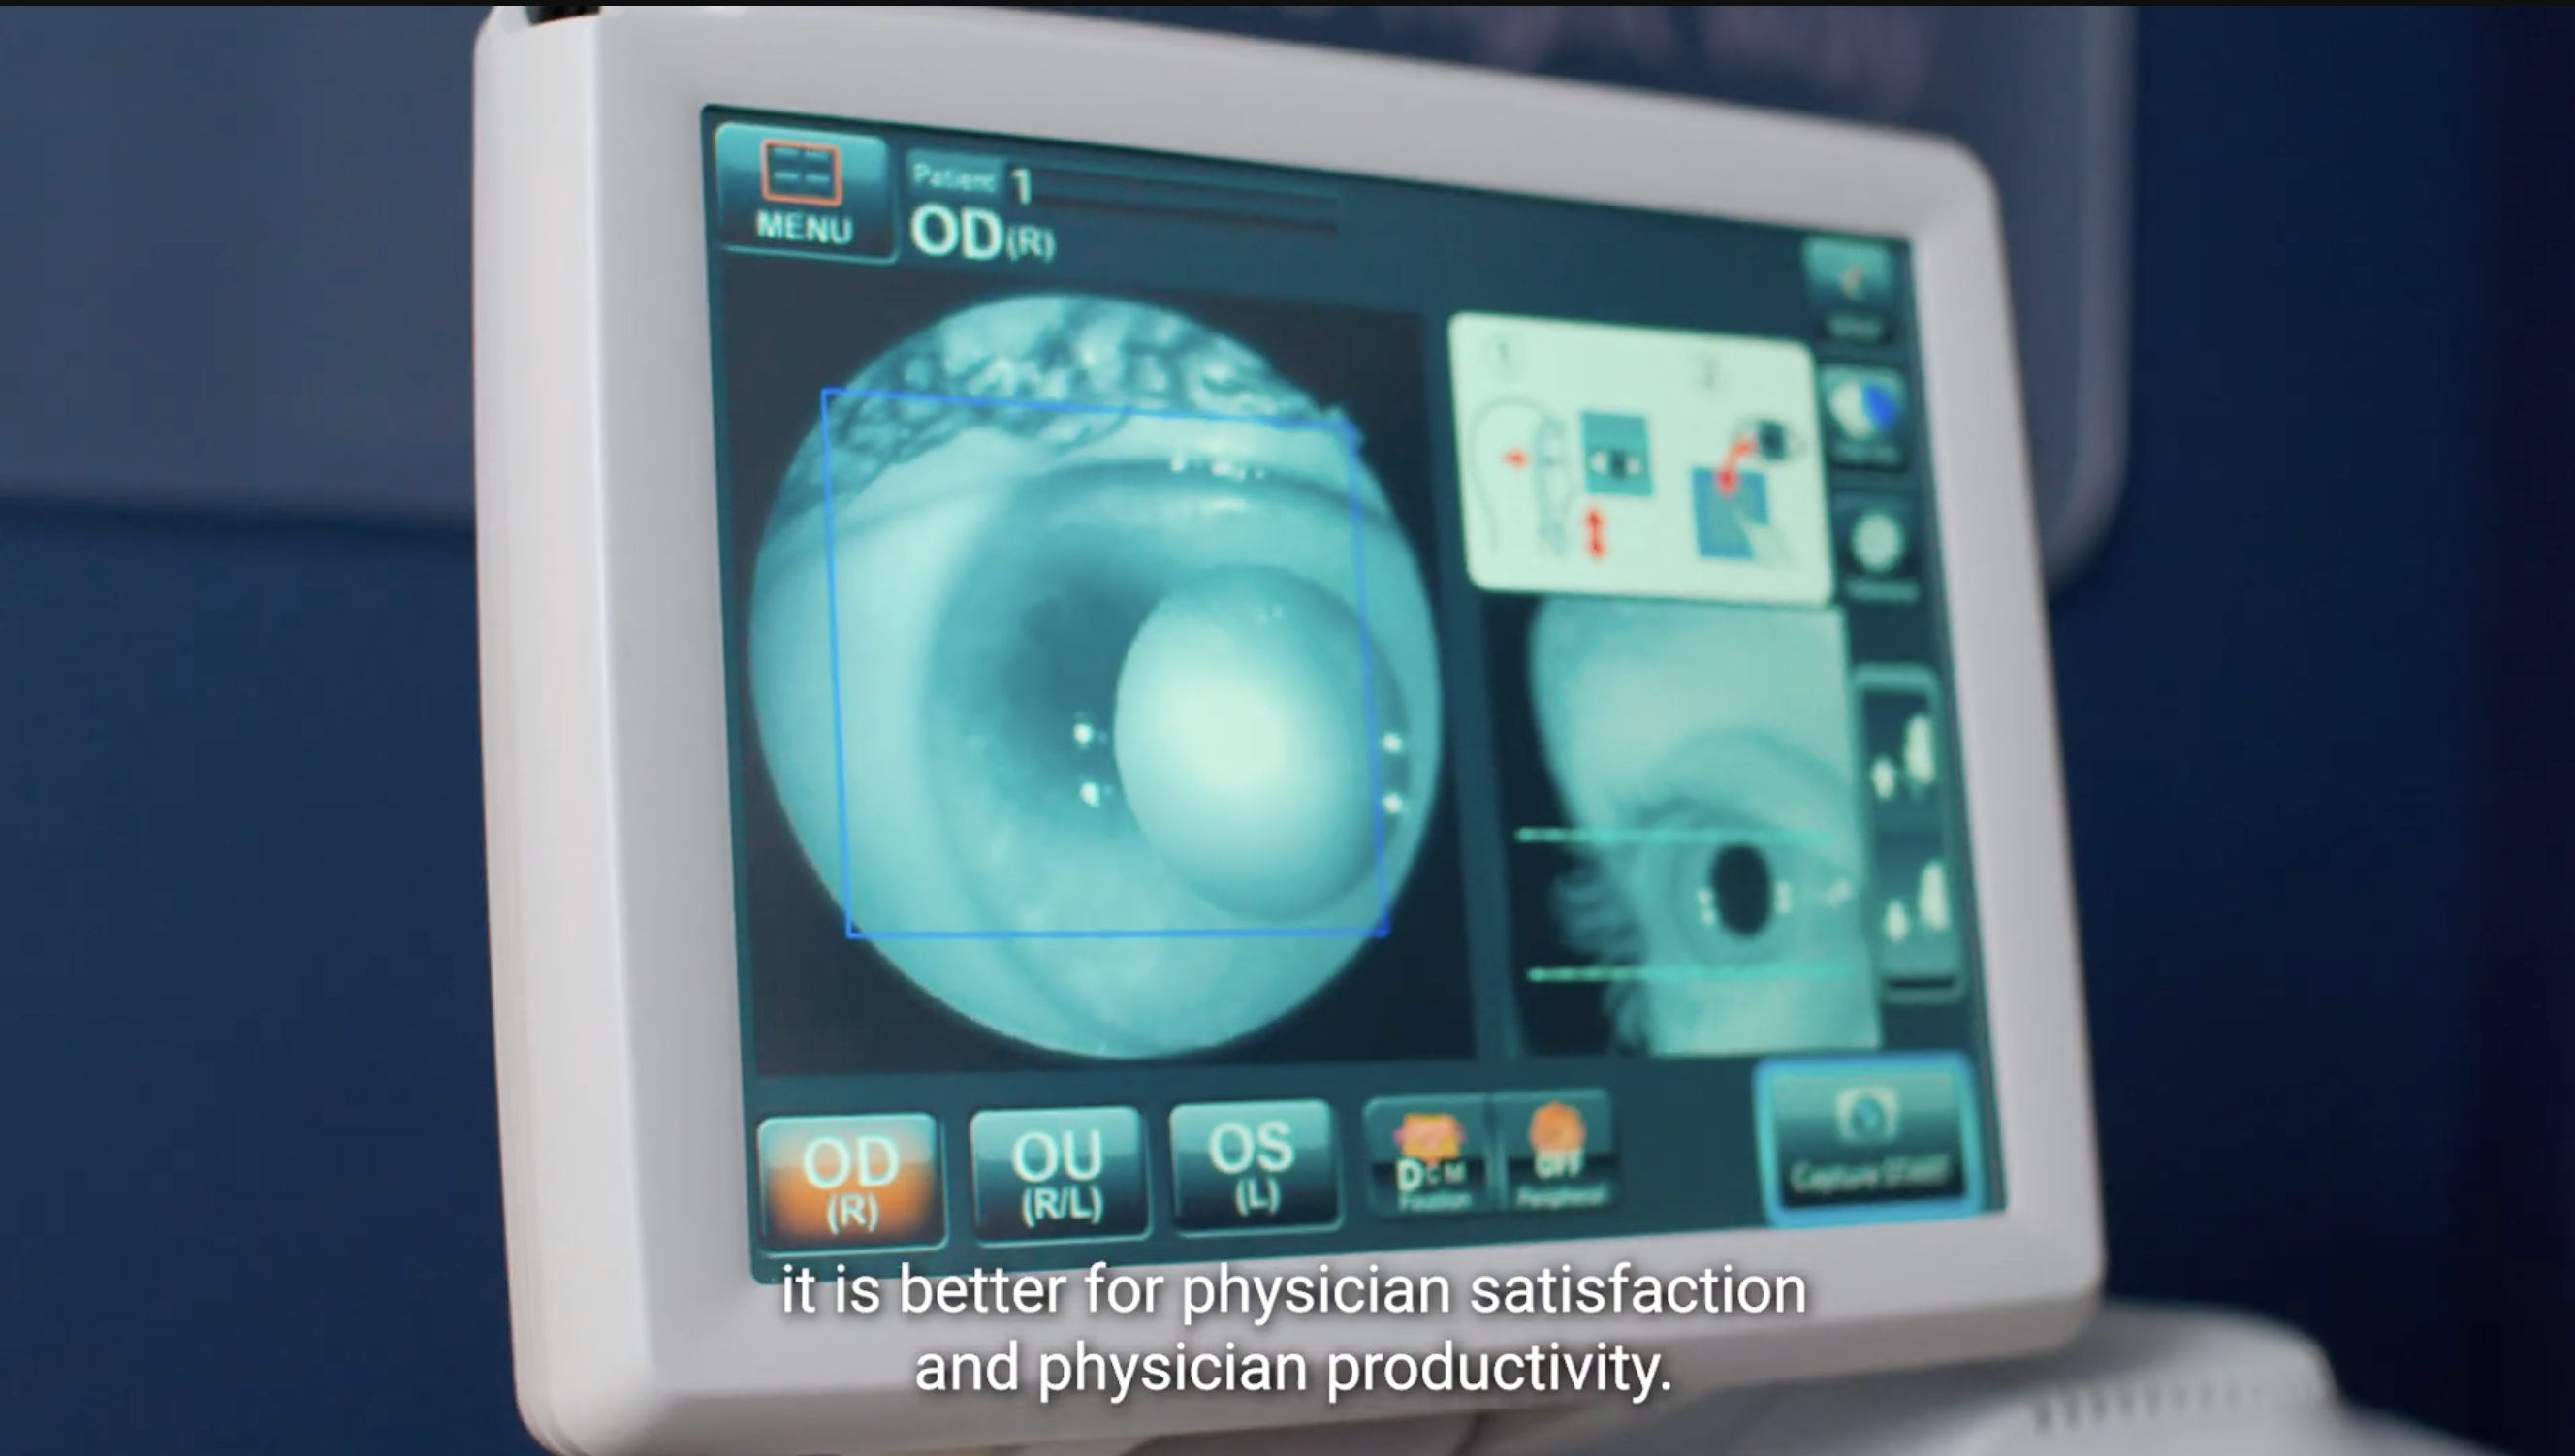
\includegraphics[width=0.8\columnwidth]{Figure1.png}
\caption{Operating interface of the Topcon camera paired with LumineticsCore. Through its graphical guidance and simple layout, the interface demonstrates usability principles such as error prevention, recognition rather than recall, and minimalist design. (Image source: Digital Diagnostics' official YouTube channel).}
\label{fig:interface}
\end{figure}

\item \textbf{Flexibility and efficiency of use: $\bigstar\bigstar\bigstar$}

The system pursues standardized efficiency rather than personalized flexibility. It does not offer shortcuts or customization options for ``advanced users.'' Its efficiency is demonstrated in the highly streamlined process and rapid analysis feedback, which perfectly aligns with its ``plug-and-play'' positioning in the primary care environment.

\item \textbf{Aesthetic and minimalist design: $\bigstar\bigstar\bigstar\bigstar$}

Based on publicly available materials, the system's interface design follows the typical style of medical software: function-first, simple, and clear. The interface retains only the essential information and controls necessary to perform the task, avoiding any extraneous elements that could distract the user.

\item \textbf{Help users recognize, diagnose, and recover from errors: $\bigstar\bigstar\bigstar\bigstar\bigstar$}

The system's mechanism for diagnosing and recovering from errors is exemplary. The ``Insufficient quality'' result is itself a clear error diagnosis, and the system provides a straightforward recovery plan: ``Resubmit or refer.'' This guides the user to take immediate and correct remedial action, forming a safe, closed-loop workflow.

\item \textbf{Help and documentation: $\bigstar\bigstar\bigstar\bigstar$}

As a medical device regulated by the FDA, providing clear documentation and training is mandatory. Digital Diagnostics provides a standardized certification training program for all operators. This ensures that all users have the basic competency to operate the system and incorporates operational standards and help documentation into their onboarding preparation.

\end{enumerate}

\subsection{Summary: User Experience and Accessibility}

The user experience of LumineticsCore can be defined as ``seamless'' and ``low cognitive load.'' It successfully transforms a complex diagnostic task that originally required expert skills into a standardized process that general healthcare staff can complete in a few simple steps.

In terms of accessibility, its contribution is twofold:

\textbf{For operators:} It enables nurses, technicians, and medical assistants without an ophthalmology background to perform fundus screening tasks, thereby broadening the range of healthcare providers who can deliver this service.

\textbf{For patients and the healthcare system:} It brings professional fundus screening services from scarce specialist centers down to community-level primary care clinics, greatly improving the accessibility of timely screening for patients with diabetes, especially in areas with limited medical resources.

\textbf{Conclusion:} The usability design of LumineticsCore is a key component of its technological success. By adhering to user-centered design principles, particularly its robust error prevention and clear communication mechanisms, it ensures that the AI's analytical capabilities can be safely and reliably unleashed in a real-world clinical environment, making it an excellent case study in usability design for medical AI.

\section{Explainability / Reverse-Engineering}

As a model based on a deep learning convolutional neural network (CNN), the internal decision-making process of LumineticsCore is inherently a ``black box.'' Its conclusions are derived from complex calculations involving millions of parameters applied to image pixels and cannot be directly explained in simple human language. However, we can ``reverse-engineer'' its working principles by creating a simplified decision model based on clinical logic, and on this basis, evaluate the transparency and comprehensibility of its output.

\subsection{Simplified Decision Tree Model}

The core task of LumineticsCore is to mimic the process of an ophthalmologist reading and grading images according to the ETDRS standard. We can simplify this complex recognition process into a conceptual decision tree, as shown in Figure~\ref{fig:decision-tree}.

\begin{figure}[htbp]
    \centering
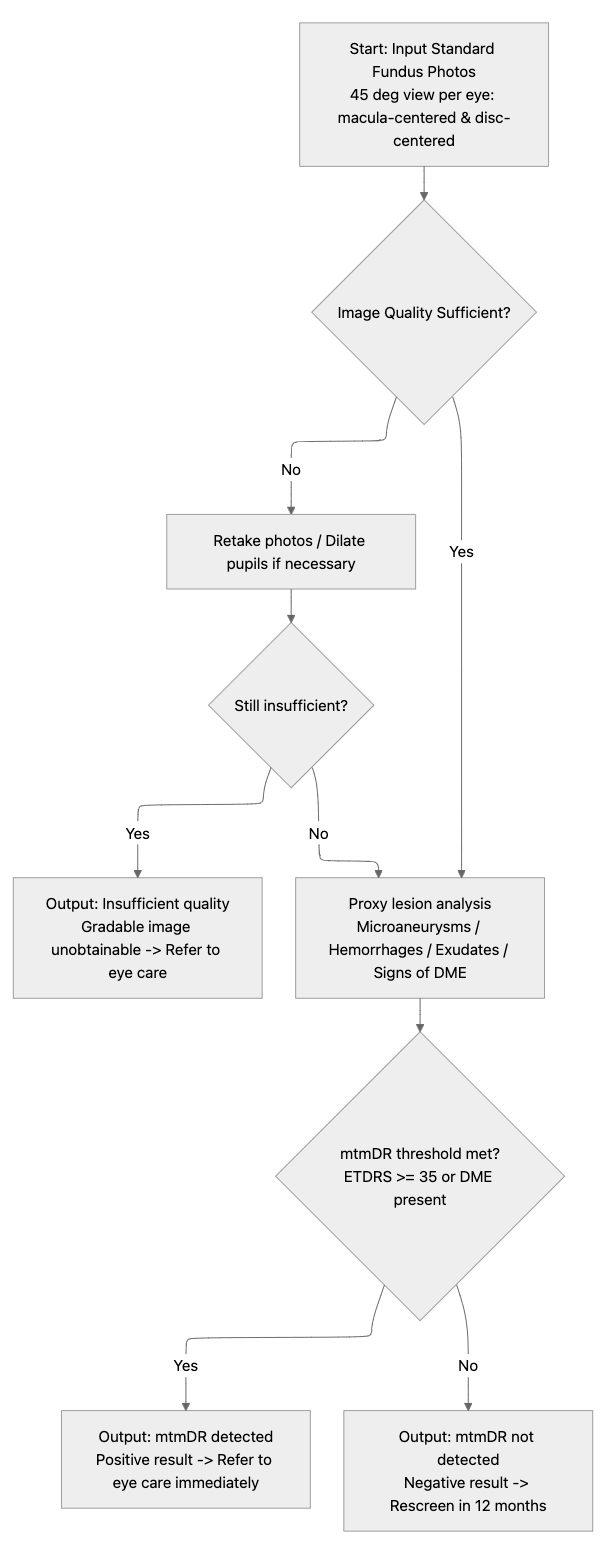
\includegraphics[width=\columnwidth]{Figure2.jpg}
\caption{Simplified decision tree model of LumineticsCore's diagnostic workflow. The system first evaluates image quality, then performs lesion analysis to determine if the mtmDR threshold is met (ETDRS $\geq$ 35 or DME present), and finally outputs one of three actionable clinical recommendations.}
\label{fig:decision-tree}
\end{figure}

\textbf{Decision Tree Logic Explanation:}

\textbf{Step 1: Image Quality Assessment}

This is the system's ``gatekeeper.'' The model first determines if the image is clear, if the field of view is standard, and if there are any obstructions. This is a prerequisite for any diagnosis. If the image quality does not meet the standard, all subsequent analysis is halted, and the system directly outputs the ``Insufficient Quality'' result.

\textbf{Step 2: Key Lesion Detection}

If the image quality is sufficient, the model begins to identify key biomarkers of diabetic retinopathy, primarily including microaneurysms, hemorrhages, hard exudates, and signs associated with diabetic macular edema (DME).

\textbf{Step 3: Severity Quantification and Aggregation}

This is the core of the decision-making process. The system does not simply ``count'' lesions; rather, it conducts a comprehensive assessment of their quantity, size, location, and other features, and compares this against the ETDRS clinical grading scale. Its final judgment is: does the sum of all detected lesions meet the threshold for ``more-than-mild diabetic retinopathy (mtmDR)'' (i.e., ETDRS level $\geq$ 35)?

\begin{itemize}
\item If not, even if a few lesions are present, the system will return a negative result as the threshold has not been met.
\item If yes, the system will return a positive result and trigger a referral recommendation.
    \end{itemize}
    
\subsection{Evaluation of Transparency and Comprehensibility}

LumineticsCore's design makes a fundamental trade-off: it sacrifices process transparency in exchange for clarity of results.

\textbf{For clinicians (operators, such as nurses/technicians):}

\textit{Comprehensibility - Extremely High:} The output is exceptionally easy to understand. Operators do not need to understand what ``hard exudates'' are; they only need to understand the clear directive to ``refer.'' This design significantly reduces cognitive load and perfectly fits the efficient, assembly-line-like workflow of a primary care setting.

\textit{Transparency - Extremely Low:} The system provides absolutely no explanation for the ``why.'' When a patient asks, ``What exactly did the AI see wrong?'' the operator cannot provide a specific answer. This may, to some extent, weaken the healthcare provider's professional authority in front of the patient and also makes it difficult for them to perform any common-sense checks or challenges to the AI's conclusion.

\textbf{For patients:}

\textit{Comprehensibility - Extremely High:} The patient receives a simple and clear next step: ``You need to see an eye care specialist'' or ``You need to be rescreened in 12 months.''

\textit{Transparency - Extremely Low:} This lack of explanation in the diagnosis may cause anxiety and distrust in patients. The experience of ``a black-box machine I don't understand says I have a problem, but it won't tell me what the problem is'' can be unsettling. Compared to a doctor who can point to a fundus photo and explain, ``Look, there is a small hemorrhage here,'' the AI's diagnosis lacks a human touch and reassuring effect, which could potentially impact the patient's adherence to the subsequent referral recommendation.

\textbf{Conclusion: A Deliberate Trade-off for a Specific Context}

The ``black-box'' nature of LumineticsCore is not a design flaw but a deliberate, strategic design trade-off made to solve a specific clinical pain point (namely, poor screening adherence). In an ideal world, an AI would be both accurate and completely transparent. However, in the real-world primary care setting, providing a detailed, expert-level explanatory report to a non-specialist nurse would not only be unhelpful but could also create risks due to misinterpretation.

Therefore, the system opts to encapsulate all complexity and output only a simple ``yes/no/retake'' signal. While this sacrifices explainability, it maximizes the system's usability and safety, ensuring that in the broadest range of scenarios, the most critical clinical decision (whether an immediate referral is needed) can be communicated and executed accurately and without error. This, in itself, is a form of transparency oriented toward safety and efficiency.

\section{Performance and Clinical Impact}

\subsection{Output Accuracy and Performance Metrics}

The accuracy of LumineticsCore is not self-proclaimed; rather, it was established in a multi-center, prospective pivotal clinical trial involving 900 subjects, through direct comparison with expert interpretations from the most authoritative independent gold standard in ophthalmology---the Wisconsin Fundus Photograph Reading Center (FPRC) \cite{abramoff2018pivotal}. The key performance metrics from this trial are as follows:

\begin{itemize}
\item \textbf{Sensitivity: 87.2\%}

\textit{Interpretation:} Sensitivity measures the ability to ``find it right.'' This means that among all patients who genuinely have ``more-than-mild diabetic retinopathy (mtmDR),'' the system successfully identified 87.2\% of them. This is a very robust level, ensuring that the vast majority of patients requiring a referral are correctly screened.

\item \textbf{Specificity: 90.7\%}

\textit{Interpretation:} Specificity measures the ability to ``rule it out right.'' This means that among all patients who were healthy or whose condition did not meet the referral criteria, the system correctly identified 90.7\% as negative. This is also a high metric, effectively preventing a large number of unnecessary referrals and reducing patient anxiety and the waste of medical resources.

\item \textbf{Imageability Rate / Gradable Image Rate: 96.1\%}

\textit{Interpretation:} In a real-world primary care environment, 96.1\% of patients were able to receive a definitive (positive or negative) diagnostic result from the system. This indicates that the system has high robustness in practical application and rarely encounters ``unanalyzable'' or invalid situations.
\end{itemize}

These data strongly demonstrate the accuracy and applicability of its output. Notably, the system successfully surpassed the success criteria set by the FDA before the trial (sensitivity $>$ 85\%, specificity $>$ 82.5\%) \cite{fda2018denovo_summary}, which was a firm requirement for receiving its De Novo authorization. Overall, its sensitivity and specificity indicate that the system has a very balanced performance, meaning its F1 Score would also be at a high level, making it suitable as a reliable clinical screening tool.

\subsection{Comparison with Clinical Guidelines and Real-World Situation}

\textbf{Comparison with Clinical Guidelines:}

The recommendation logic of LumineticsCore is highly consistent or compatible with the diabetic eye screening guidelines published by authoritative bodies such as the American Academy of Ophthalmology (AAO) and the American Diabetes Association (ADA). For example, its recommendation to ``rescreen in 12 months for a negative finding'' is consistent with the recommended annual follow-up interval in guidelines for most patients with no or mild DR; while guidelines also mention that for patients who are persistently negative with good metabolic control, the follow-up interval can be extended to 1-2 years. Similarly, its threshold for ``referral for a positive finding'' (more-than-mild DR) aligns with the core recommendation in guidelines that ``when moderate or more severe DR or DME is present, it must be managed or more closely followed by an ophthalmologist.'' Therefore, the system can be seen as an effective tool for automating existing best clinical practices. It is not creating new medical knowledge, but rather implementing existing, best clinical practices in a more efficient and accessible way at the primary care level.

\textbf{Comparison with the Real-World Situation:}

This is precisely where LumineticsCore demonstrates its significant clinical impact. In the traditional ``real-world situation,'' after a primary care physician identifies that a patient needs a fundus screening, they can only issue a referral. The patient must then schedule an appointment with an ophthalmologist on their own, bear additional costs for time and transportation, and often face a long wait. Adherence to this process is extremely low.

In contrast, LumineticsCore creates an entirely new ``point-of-care diagnostic'' scenario. A recent randomized controlled trial involving adolescents strikingly revealed this difference \cite{wolf2024autonomous}:

\begin{itemize}
\item \textbf{Conventional referral group:} Only 22\% of patients completed their eye exam within 6 months.
\item \textbf{AI-assisted screening group:} The completion rate for eye exams was 100\% within 6 months.
\end{itemize}

\textbf{Conclusion:} The clinical quality of LumineticsCore lies not only in its diagnostic accuracy of around 90\% but, more importantly, in its ability to increase the screening completion rate from 22\% to 100\%. From a public health perspective, the clinical benefit of using a tool with an approximate 13\% risk of missed diagnosis (100\% - 87.2\% sensitivity) to cover 100\% of the target population far outweighs the current situation of using a perfect tool (assuming diagnosis by a top expert) that only covers 22\% of the population. It solves the most critical bottleneck in the screening process---patient loss to follow-up and delays---and this is its most significant clinical impact.

\section{Reflection and Recommendations}

\subsection{Reflection on Overall Performance}

Based on a multi-dimensional evaluation of the LumineticsCore system, it can be concluded that this solution is not only a technological breakthrough but also a highly successful example of real-world clinical deployment. Its performance goes well beyond a simple image-classification tool; its true value lies in a deep understanding of---and deliberate redesign for---existing care pathways.

The system's core strength is its end-to-end, integrated design. It begins with a solid knowledge base---high-quality data aligned with expert consensus and validated through large, prospective clinical studies \cite{abramoff2018pivotal}; it then safely delivers complex AI analytics to non-specialists via a streamlined and highly error-preventive user interface \cite{fda2018denovo_summary}; and it ends with clear, immediately actionable clinical instructions that directly address the major pain points in traditional screening---poor adherence and workflow delays \cite{wolf2024autonomous}. Although its ``black-box'' nature sacrifices process transparency, this represents a considered trade-off to maximize usability and safety in primary care. Overall, LumineticsCore merits an assessment of ``excellent,'' not only for accurately answering ``Does this patient have referable disease?'' but, more importantly, for solving the systemic question: ``How do we ensure the patient actually completes necessary screening?''

\subsection{Ethical Issues, Potential Improvements, and Recommendation}

\textbf{Ethical issues.}

Despite strong performance, several ethical challenges require attention:

\begin{enumerate}
\item \textbf{Accountability.} In the event of a false-negative (missed disease) leading to harm, responsibility becomes complex. Is the accountable party the algorithm developer (Digital Diagnostics), the clinic deploying the device, or the operator who failed to appreciate the AI's limitations? Clear legal and ethical frameworks remain to be refined.

\item \textbf{Equity.} On one hand, LumineticsCore advances equity by bringing specialist-level screening to the front lines. On the other hand, the costs of camera and software may pose an access barrier for resource-constrained clinics, potentially creating a new ``digital divide.''

\item \textbf{Provider--patient communication.} The ``black-box'' property complicates communication. When an opaque algorithm renders a diagnosis, clinicians must still manage patient anxiety and build trust---new requirements for users of autonomous AI.
\end{enumerate}

\textbf{Potential improvements.}

\begin{enumerate}
\item \textbf{``Lite'' explainability.} Future versions could explore lightweight, operator-friendly explanations (e.g., a simple heatmap highlighting regions of interest) to support patient communication without increasing cognitive load.

\item \textbf{Expanded diagnostic scope.} The current model targets DR only. Training for additional common retinal diseases (e.g., glaucoma, age-related macular degeneration, AMD) would substantially increase both clinical and economic value.

\item \textbf{Hardware compatibility.} Reducing reliance on a specific Topcon model and supporting a broader range of fundus cameras would lower adoption barriers and accelerate diffusion.
\end{enumerate}

\textbf{Limitations and cautious extrapolation.}

While LumineticsCore performs strongly, broader deployment should recognize the boundaries of the current evidence base.

\begin{itemize}
\item \textbf{Limits of evidence extrapolation.} The randomized trial in a multi-ethnic youth cohort offers strong corroboration that AI can dramatically improve screening adherence, but the study population differs from the adult indication ($\geq$22 years). The system's diagnostic accuracy in adolescents therefore warrants further dedicated validation \cite{wolf2024autonomous}.

\item \textbf{Challenges in real-world transferability.} The pivotal trial's performance benefited from the specified Topcon camera and a standardized workflow. In routine practice, heterogeneity in equipment, operator training, and workflow integration may introduce performance drift, especially in gradability \cite{fda2018denovo_summary, abramoff2018pivotal}.

\item \textbf{Re-validation after model updates.} As a machine-learning system, the algorithm may evolve over time. The FDA's PCCP framework provides a path, but clinical users should ensure the deployed version is aligned with the version(s) underpinning key published evidence, and that substantive updates are supported by fresh real-world data \cite{fda2018denovo_summary, abramoff2018pivotal}.
\end{itemize}

\textbf{Recommendation.}

I strongly recommend deploying LumineticsCore in primary-care and endocrinology settings.

This recommendation comes with an essential caveat: the system should not be treated as a standalone ``box,'' but rather integrated into a complete clinical workflow, including standardized operator training and certification, a communication plan for discussing positive results with patients, and a reliable, well-functioning referral pathway to ophthalmic specialists.

\subsection{Conclusion on Its Role in Improving Healthcare}

LumineticsCore's true contribution to healthcare is not merely an accurate screening tool; it represents a scalable, new paradigm for preventive chronic-disease management.

It compellingly demonstrates that the greatest value of AI in healthcare may not be assisting top specialists with rare, complex diagnostics, but rather embedding standardized, high-quality, foundational services---automated and tireless---at the very frontline of care. It addresses fundamental issues of efficiency, workflow, adherence, and access.

In the end, LumineticsCore is not only a milestone for ophthalmic AI but also a blueprint for autonomous diagnostic AI at large. It points to a future in which carefully designed, human-centered AI systems extend expert knowledge to every setting where it is needed---realizing the goals of equity and universal benefit in healthcare.

%%
%% Bibliography
%%
\bibliographystyle{ACM-Reference-Format}
\bibliography{references}

\end{document}
